\section{Tests}

We designed both manually designed three different worlds with increasing complexity and 1000 random worlds with random complexity.

\subsection{Manually Created Worlds}

The first example \texttt{data/examples/test1} is a simple world with only one Machine and one Petition:

\texttt{InitialState=Robot-location(o1);Machine(o16,1);Petition(o26,1);Robot-free; Steps(0);
GoalState=Robot-location(o7);Served(o26);}

The world \texttt{data/examples/test1} can be seen in figure \ref{fig:manworlds} (a).

\begin{figure}[!ht]
\centering     %%% not \center
\subfigure[test1]{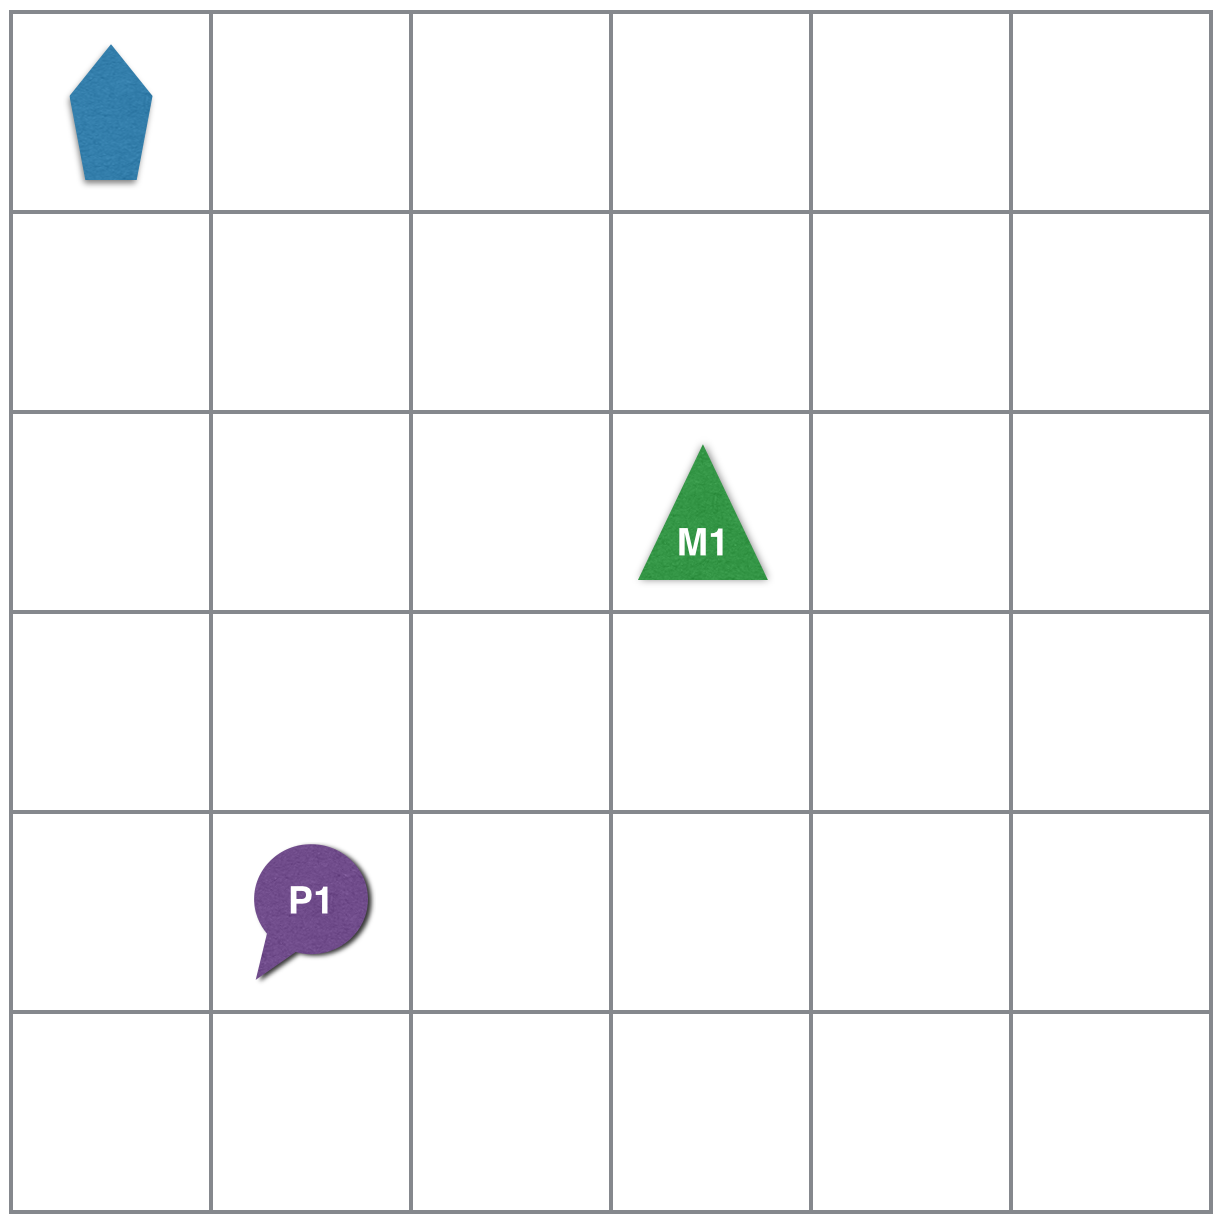
\includegraphics[width=40mm]{img/w1}}
\subfigure[test2]{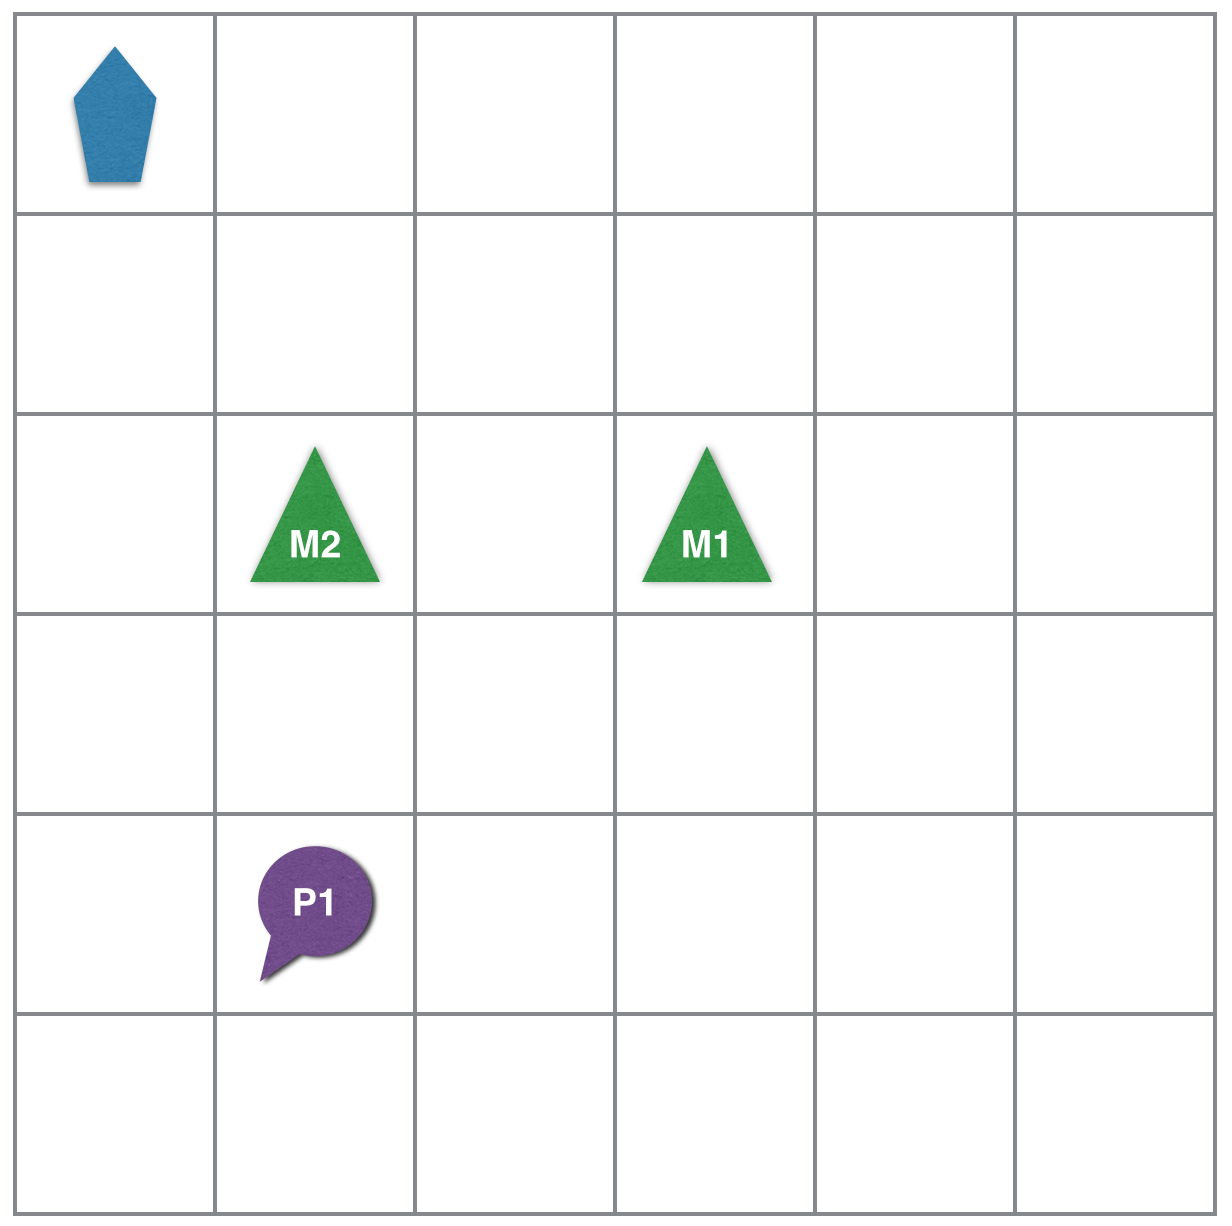
\includegraphics[width=40mm]{img/w2}}
\subfigure[test3]{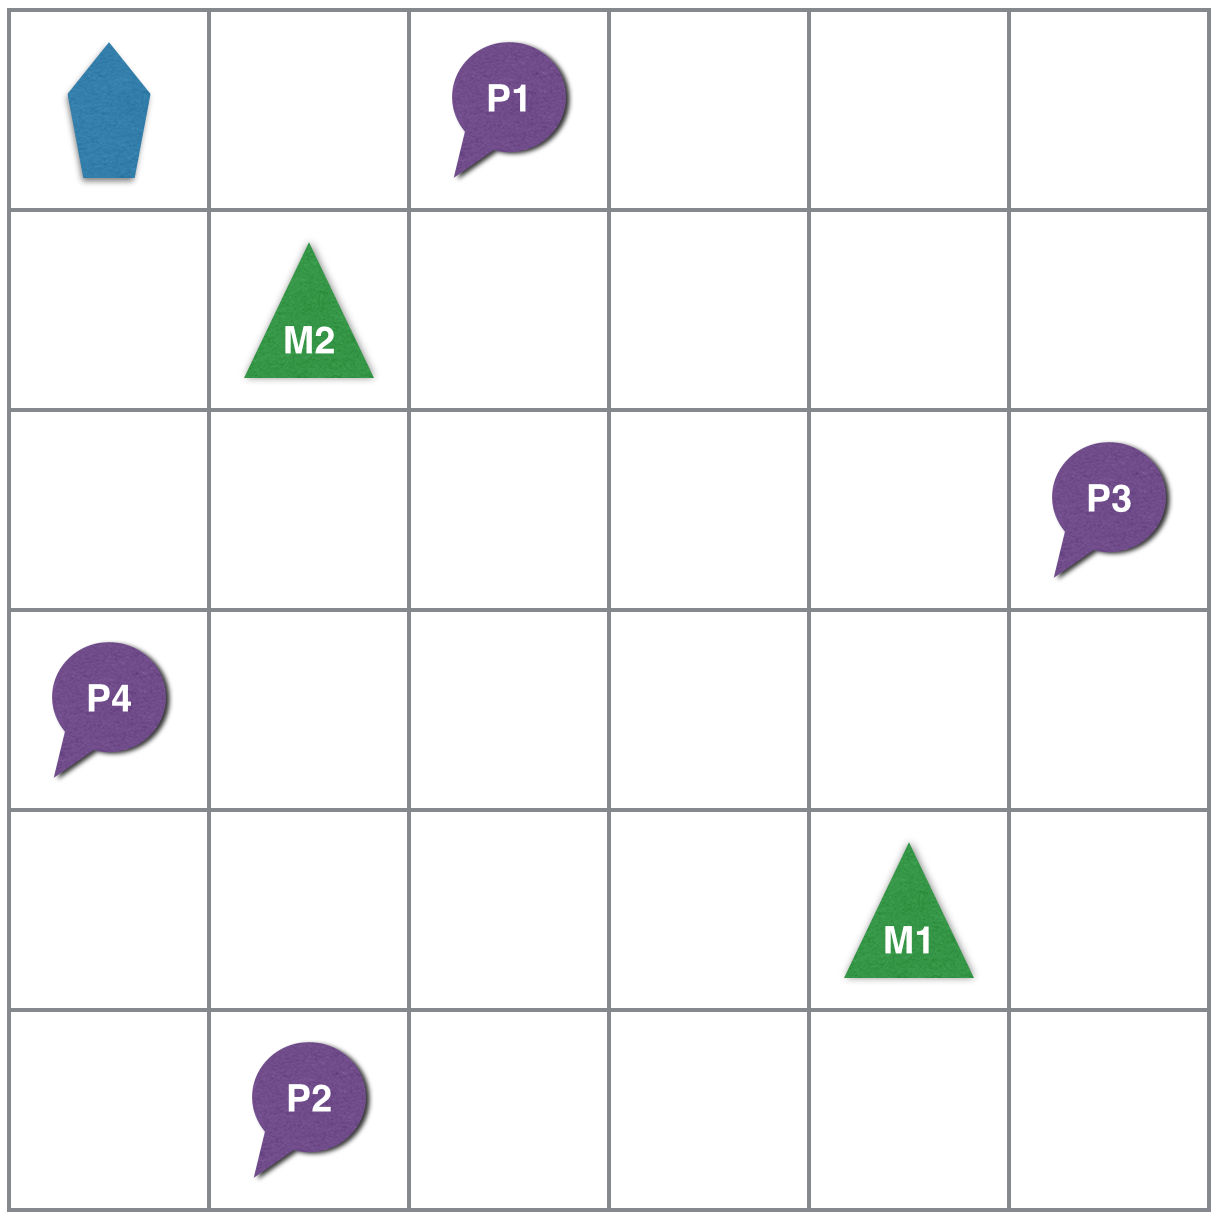
\includegraphics[width=40mm]{img/w3}}
\caption{Manually created examples}
\label{fig:manworlds}
\end{figure}

The second example \texttt{data/examples/test2} is a more complex world with now two Machines and one Petition:

\texttt{InitialState=Robot-location(o1);Machine(o16,1);Machine(o14,1);Petition(o26,1); Robot-free; Steps(0);
GoalState=Robot-location(o7);Served(o26);}

The world \texttt{data/examples/test2} can be seen in figure \ref{fig:manworlds} (b).

The third example \texttt{data/examples/test2} is even more complex  with two Machines and now four Petitions:

\texttt{InitialState=Robot-location(o1);Machine(o29,1);Machine(o8,1);Petition(o3,1); Petition(o32,1);Petition(o18,1);Petition(o19,1);Robot-free; Steps(0); 
GoalState= Robot-location(o7);Served(o3);Served(o32);Served(o18);Served(o19);}

The world \texttt{data/examples/test3} can be seen in figure \ref{fig:manworlds} (c).


\subsection{Automatically created worlds}

We created 1000 random worlds. Each of these worlds has between 3 and 9 petitions (at least one for each possible $n$) and between 3 and 9 machines (at least one for each possible $n$). The generated examples are attached to this report, see appendix \ref{app:included}.